
\RequirePackage{filecontents}

\documentclass[11pt]{article}

\usepackage[left=1in, right=1in, top=1in, bottom=1in]{geometry}

\usepackage{mathptmx} % for font
\usepackage{listings} % for code lstlisting
\usepackage{amsmath} % for \implies arrow
\usepackage{float} % for putting tables H
\usepackage{changepage} % for centering table with larger margin
\usepackage{multirow} % for multirow in tables

%\pagenumbering{gobble}

\linespread{1.3} % for "double" spacing

\usepackage{biblatex}
\addbibresource{refs.bib}

% wrap figure next to text
\usepackage{graphicx,wrapfig,lipsum}

% for custom margin sizes for code
\def\changemargin#1#2{\list{}{\rightmargin#2\leftmargin#1}\item[]}
\let\endchangemargin=\endlist 

% make figure bold
\usepackage[labelfont=bf]{caption}

\usepackage{booktabs} % for toprule midrule etc

\usepackage{floatflt} % for table next to text

\renewcommand*{\bibfont}{\small} % for bibliography font

\author{Jennifer Garner}
\date{\today}
\title{Final Project: Association Rules for Drug Reviews \& Clustering of Drug Data using Molecular Fingerprints \\ \small CSE*780 Winter 2019}

\begin{document}

\maketitle
\tableofcontents

\newpage
\section{Programs Used}

This project was completed using a combination of R (version 3.5.1 (2018-07-02) -- ``Feather Spray") and Python (version 3.6.8 |Anaconda, Inc.| (default, Dec 30 2018, 01:22:34)) on Linux (Ubuntu 18.10). Specific packages/libraries were used as specified in the text. All code, data, images, etc. generated for this project can be found at the github repository: \url{https://github.com/PeaWagon/cse780-project}.

% Description of data including source, details on variables, relationships between variables, descriptive analyses, etc. [10 marks]

\section{Original Dataset}

The original dataset was taken from the UCI Machine Learning Repository \cite{dataset-web}\cite{paper-analysis}. The data was scraped from the Drugs.com website for the purpose of performing sentiment analysis on user satisfaction with pharmaceutical drugs. Each entry represents a user review with 6 variables: drugName, condition (what drug was used to treat), review (user's text review), rating (out of 10, for overall user satisfaction), date (review was made, 2008-2017), and usefulCount (how many people found the review useful). From \textbf{Table \ref{orig-data}}, the majority of drug ratings are positive ($\geq 7$).

\begin{table}[H]
\centering
\begin{tabular}{llllll}
\toprule
\textbf{\# entries} & \textbf{\# conditions} & \textbf{\# drugs} & \textbf{\% rating \textless{}= 4} & \textbf{\% 4 \textless rating \textless 7} & \textbf{\% rating \textgreater{}= 7} \\
\midrule
215063              & 836                    & 3654              & 25                                & 9                                          & 66      \\
\bottomrule
\end{tabular}
\caption{Some summary data for the original dataset. Adapted from \cite{paper-analysis}.}
\label{orig-data}
\end{table}

\section{Pubchem Dataset}

A subset of the data was sorted by querying the Pubchem online database \cite{pubchem}; if a drug could be found in Pubchem, then the entry was kept. Each Pubchem chemical has a cid (chemical identifier); some drugs were linked to the same cid, because they have the same active ingredient. 

\begin{table}[H]
    \centering
    \begin{tabular}{cccc}
    \toprule
\textbf{\# Original Drugs} & \textbf{\# Pubchem Drugs} & \textbf{\# Non-Pubchem Drugs} & \textbf{\# Duplicate Drugs} \\
\midrule
3654* & 1370 & 1171 & $\sim$1113-1130 \\
\bottomrule
\multicolumn{4}{c}{\footnotesize{* this is the number of drugs reported in \cite{paper-analysis}; however, 3671 unique entries were found in the original dataset.}}
    \end{tabular}
    \caption{Comparison of numbers of available drugs in Pubchem versus how many were in the original database. Arguably, the number of drugs considered in the Pubchem subset is 1370+duplicates, except only 1370 of them represent unique chemical structures.}
    \label{drugs-table}
\end{table}



% Description of the problem being addressed. [4 marks]

\section{Purpose of Report}

The purpose of this project will be to use the drug dataset to:
\begin{itemize}
    \item use clustering analysis to determine the efficacy of different fingerprint methods in separating drug molecules
    \item compare linkages for hierarchical clustering and find clusters of drugs
    \item determine if review length and/or drug rating is correlated with the type of drug or condition treated using association rules analysis 
\end{itemize}

% Description of the techniques used, including the rationale for the choice of parameters, etc. [10 marks]

% Descriptions of results, both in technical terms and in the context of the data. [12 marks]

\section{Clustering Analysis}

\subsection{Preparation of Data - Molecular Fingerprints}

Molecules can be given a fingerprint, and the similarity between two fingerprints can be used as a measure of molecule similarity. Fingerprints are generated by analysing the connectivity within a molecule and the types of atoms present. For example, a molecule can be represented using a SMILES (simplified molecular-input line-entry system) string, and its fragments can be analysed by making SMARTS (SMILES arbitrary target specification) queries. The SMILES string for caffeine is $CN1C=NC2=C1C(=O)N(C(=O)N2C)C$, and the SMARTS query for a primary alcohol would be $[OX2H][CX4H2;!\$(C([OX2H])[O,S,#7,#15])]$.

Using the Python library PubChemPy \cite{pcp}, SMILES strings for the drug molecules were scraped from Pubchem. Then, the Python library Pybel \cite{pybel}\cite{openbabel} was used to assign a fingerprint to each drug/SMILES string that was found in Pubchem. A similarity matrix was generated by calculating the Tanimoto coefficient for each pair of drugs. 4 similarity matrices were produced, using the four fingerprints available in Pybel: FP2, FP3, FP4, and MACCS \cite{fingerprints}. Dissimilarity matrices were generated for each fingerprint by subtracting each similarity value from 1, such that identical molecules have a distance of 0 and dissimilar molecules have a maximal distance of 1.

\subsection{Clustering Methods}

Some clustering methods covered this term include: agglomerative hierarchical clustering, kmeans clustering, kmedoids clustering, and model-based clustering. Kmeans and model-based (i.e. using Mclust) clustering are not suitable analyses for the fingerprint data, as they require a data frame (and not a dissimilarity matrix) as input. Instead, the R function hclust (hierarchical clustering) and the pam (partitioning around medoids - kmedoids clustering) function from the R-package cluster \cite{r-cluster} were used, since these allow for a dissimilarity matrix to be input.

Agglomerative hierarchical clustering is a bottom-up approach, where each drug is first placed in its own cluster and then joined to the nearest other drug/cluster until one cluster remains. Usually, Euclidean and Manhattan distance metrics are used to determine the closeness of to observations; however, the distance metric used here is the Tanimoto coefficient (also called the Jaccard distance). The Jaccard distance is defined as $ J(X,Y) = 1 - \frac{X\cap Y}{X\cup Y}$ for two fingerprints $X$ and $Y$.

The linkage, or how clusters A and B are joined, can be determined using several methods, including: complete, single, average, and Ward \cite{ward}, as described by:

\noindent\textbf{Complete:} $d(A,B) = \limits_{x\in A, y\in B}^{\text{\textbf{\hspace{0.25cm}max}}} d(x,y)$, \textbf{Single:} $d(A,B) = \limits_{x\in A, y\in B}^{\text{\textbf{\hspace{0.25cm}min}}} d(x,y)$, \textbf{Average:} $d(A,B) = \frac{1}{|A||B|} \sum\limits_{x\in A}\sum\limits_{y\in B} d(x,y)$

\noindent Thus, the complete, single, and average linkages determine the biggest, smallest, and average distances (respectively) between any two data points, one from cluster A and the other from cluster B.

After clustering the data using agglomerative hierarchical clustering, a dendogram (\textbf{Figure \ref{dendograms}}) can be produced, where the height is directly proportional to the distance between the clusters. A number of cuts can be specified; cutting the dendogram in n places produces n clusters. If the data is labelled, then the cluster results for n cuts can be compared to the n labels. The dataset used in this project does not contain labels, so it is part of the analysis to determine a suitable number of cuts for good clustering of drug molecules.

\begin{figure}[H]
    \centering
    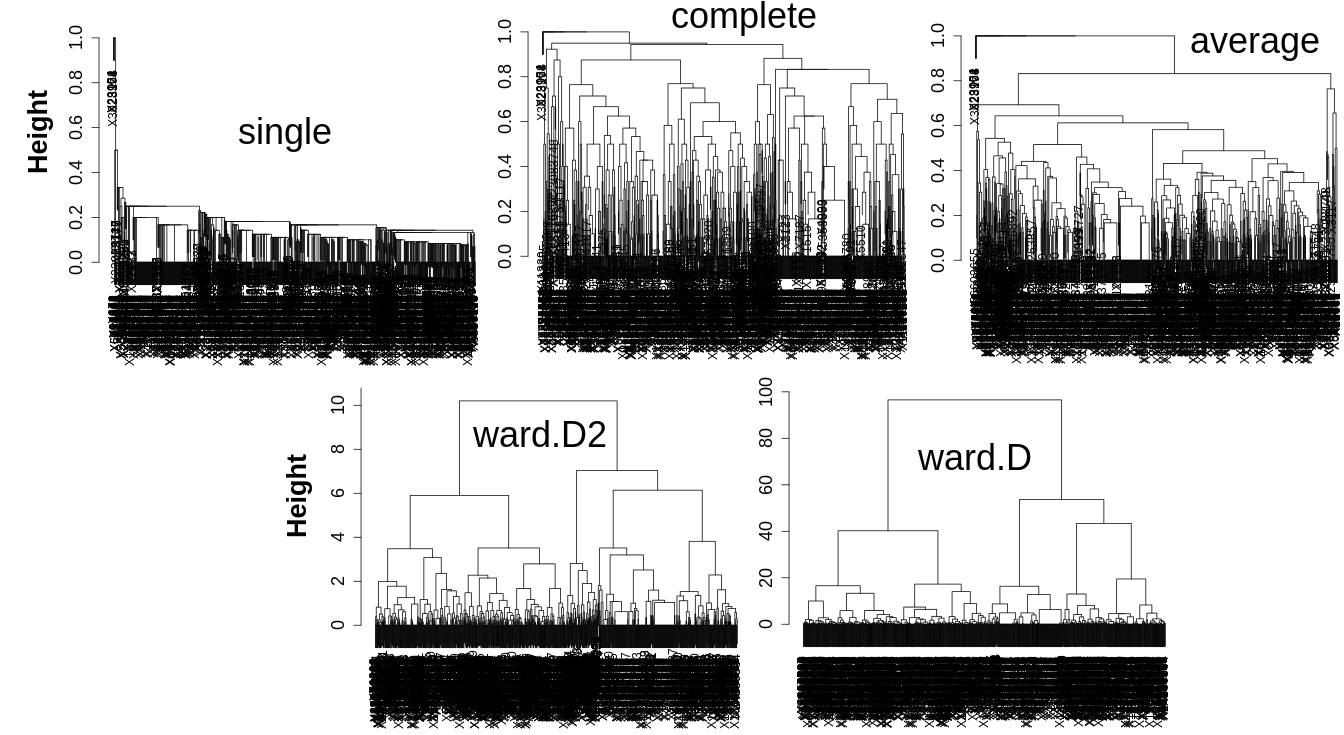
\includegraphics[width=\textwidth]{fp3_hclust.png}
    \caption{Example dendograms for 5 linkages as determined by clustering the FP3 fingerprint dissimilarity matrix using the hclust function in R.}
    \label{dendograms}
\end{figure}

Kmeans and Kmedoids are partitioning methods that work well for spherical clusters. k cluster centres are used to cluster data, and the goal is to reduce the distance for all points from a centre point. Compared to agglomerative hierarchical clustering, partitioning methods require the user to know how many clusters to make ahead of time. Kmeans clustering assigns a point X in n-dimensional space to be the centre of each cluster, whereas kmedoids clustering assigns a data point from each cluster to be the centre of the cluster.

To determine the number of clusters (value for k), a silhouette plot (\textbf{Figure \ref{silhouettte-plot}}) can be generated using the silhouette function from the cluster R-package \cite{r-cluster}. The silhouette plot shows values between -1 and 1 for each of the fingerprints, sorted by cluster. The width of the silhouette indicates how close each data point is to neighbouring clusters, where 1 is well-separated, 0 is on the boundary with other clusters, and a negative value indicates that the data point may be in the wrong cluster. The average silhouette width is therefore indicative of how well the clusters are separated from one-another, and can be used to choose a value for k.

\begin{figure}[H]
    \centering
    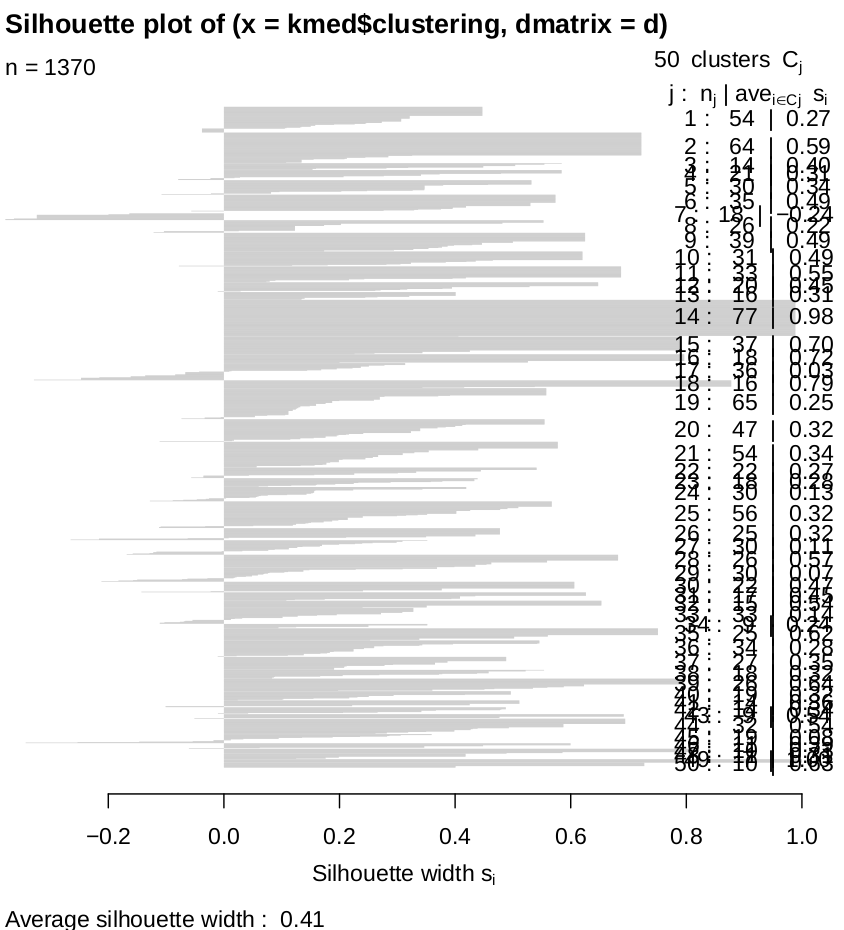
\includegraphics[width=0.75\textwidth]{silhouette_kmed_fp3.png}
    \caption{Silhouette plot of the FP3 fingerprint data as generated for 50 kmedoids clusters.}
    \label{silhouettte-plot}
\end{figure}

To compare clustering results, a contingency table can be generated. A contingency table is similar to an nxn matrix, where n is the number of clusters, except it is buffered by a summation row (at the bottom) and a summation column (on the right). The diagonals of the table represent counts from method X and method Y that both sorted into the same ith cluster (example: if $n_{11} = 3$, then 3 data points were sorted into cluster 1 for both methods X and Y). The off-diagonals represent cases where the two methods did not place data points in the same cluster. ARI accounts for random chance that may place the data points in the same clusters for methods X and Y. The rand index is a value between 0 and 1, where 1 is perfect agreement for the methods, and 0 represents agreement under random chance.

\begin{figure}[H]
    \centering
    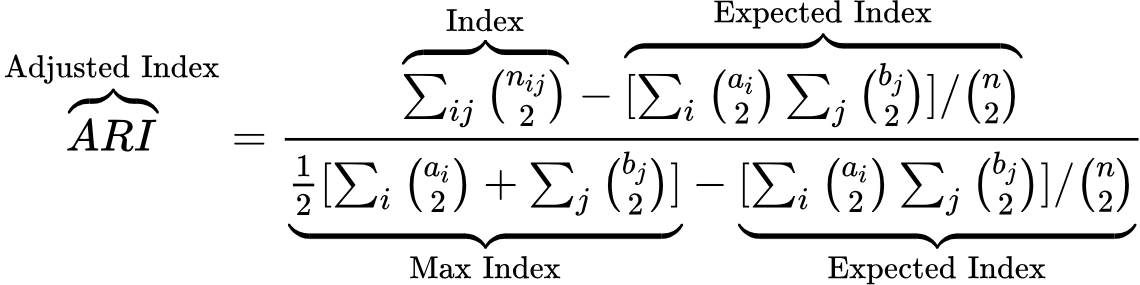
\includegraphics[width=0.65\textwidth]{ari-formula.png}
    \caption{Formula for Adjusted Rand Index (or corrected rand = crand index). Figure taken from the Wikipedia page \cite{ari-formula}.}
    \label{fig:my_label}
\end{figure}

Variation of information (VI) is another way of comparing clustering results. Given the clustering results for two methods X and Y for n clusters, the VI index is given by:

$VI = -\sum\limits_{ij}r_{ij} \left(log(r_{ij}/p_i) + log(r_{ij}/q_j)\right)$, where $p_i = |X_i|/n \text{, } q_j = |Y_j|/n \text{, and } r_{ij} = |X_i \cap Y_j|/n$

\subsection{Clustering Results}

\begin{figure}[H]
\centering
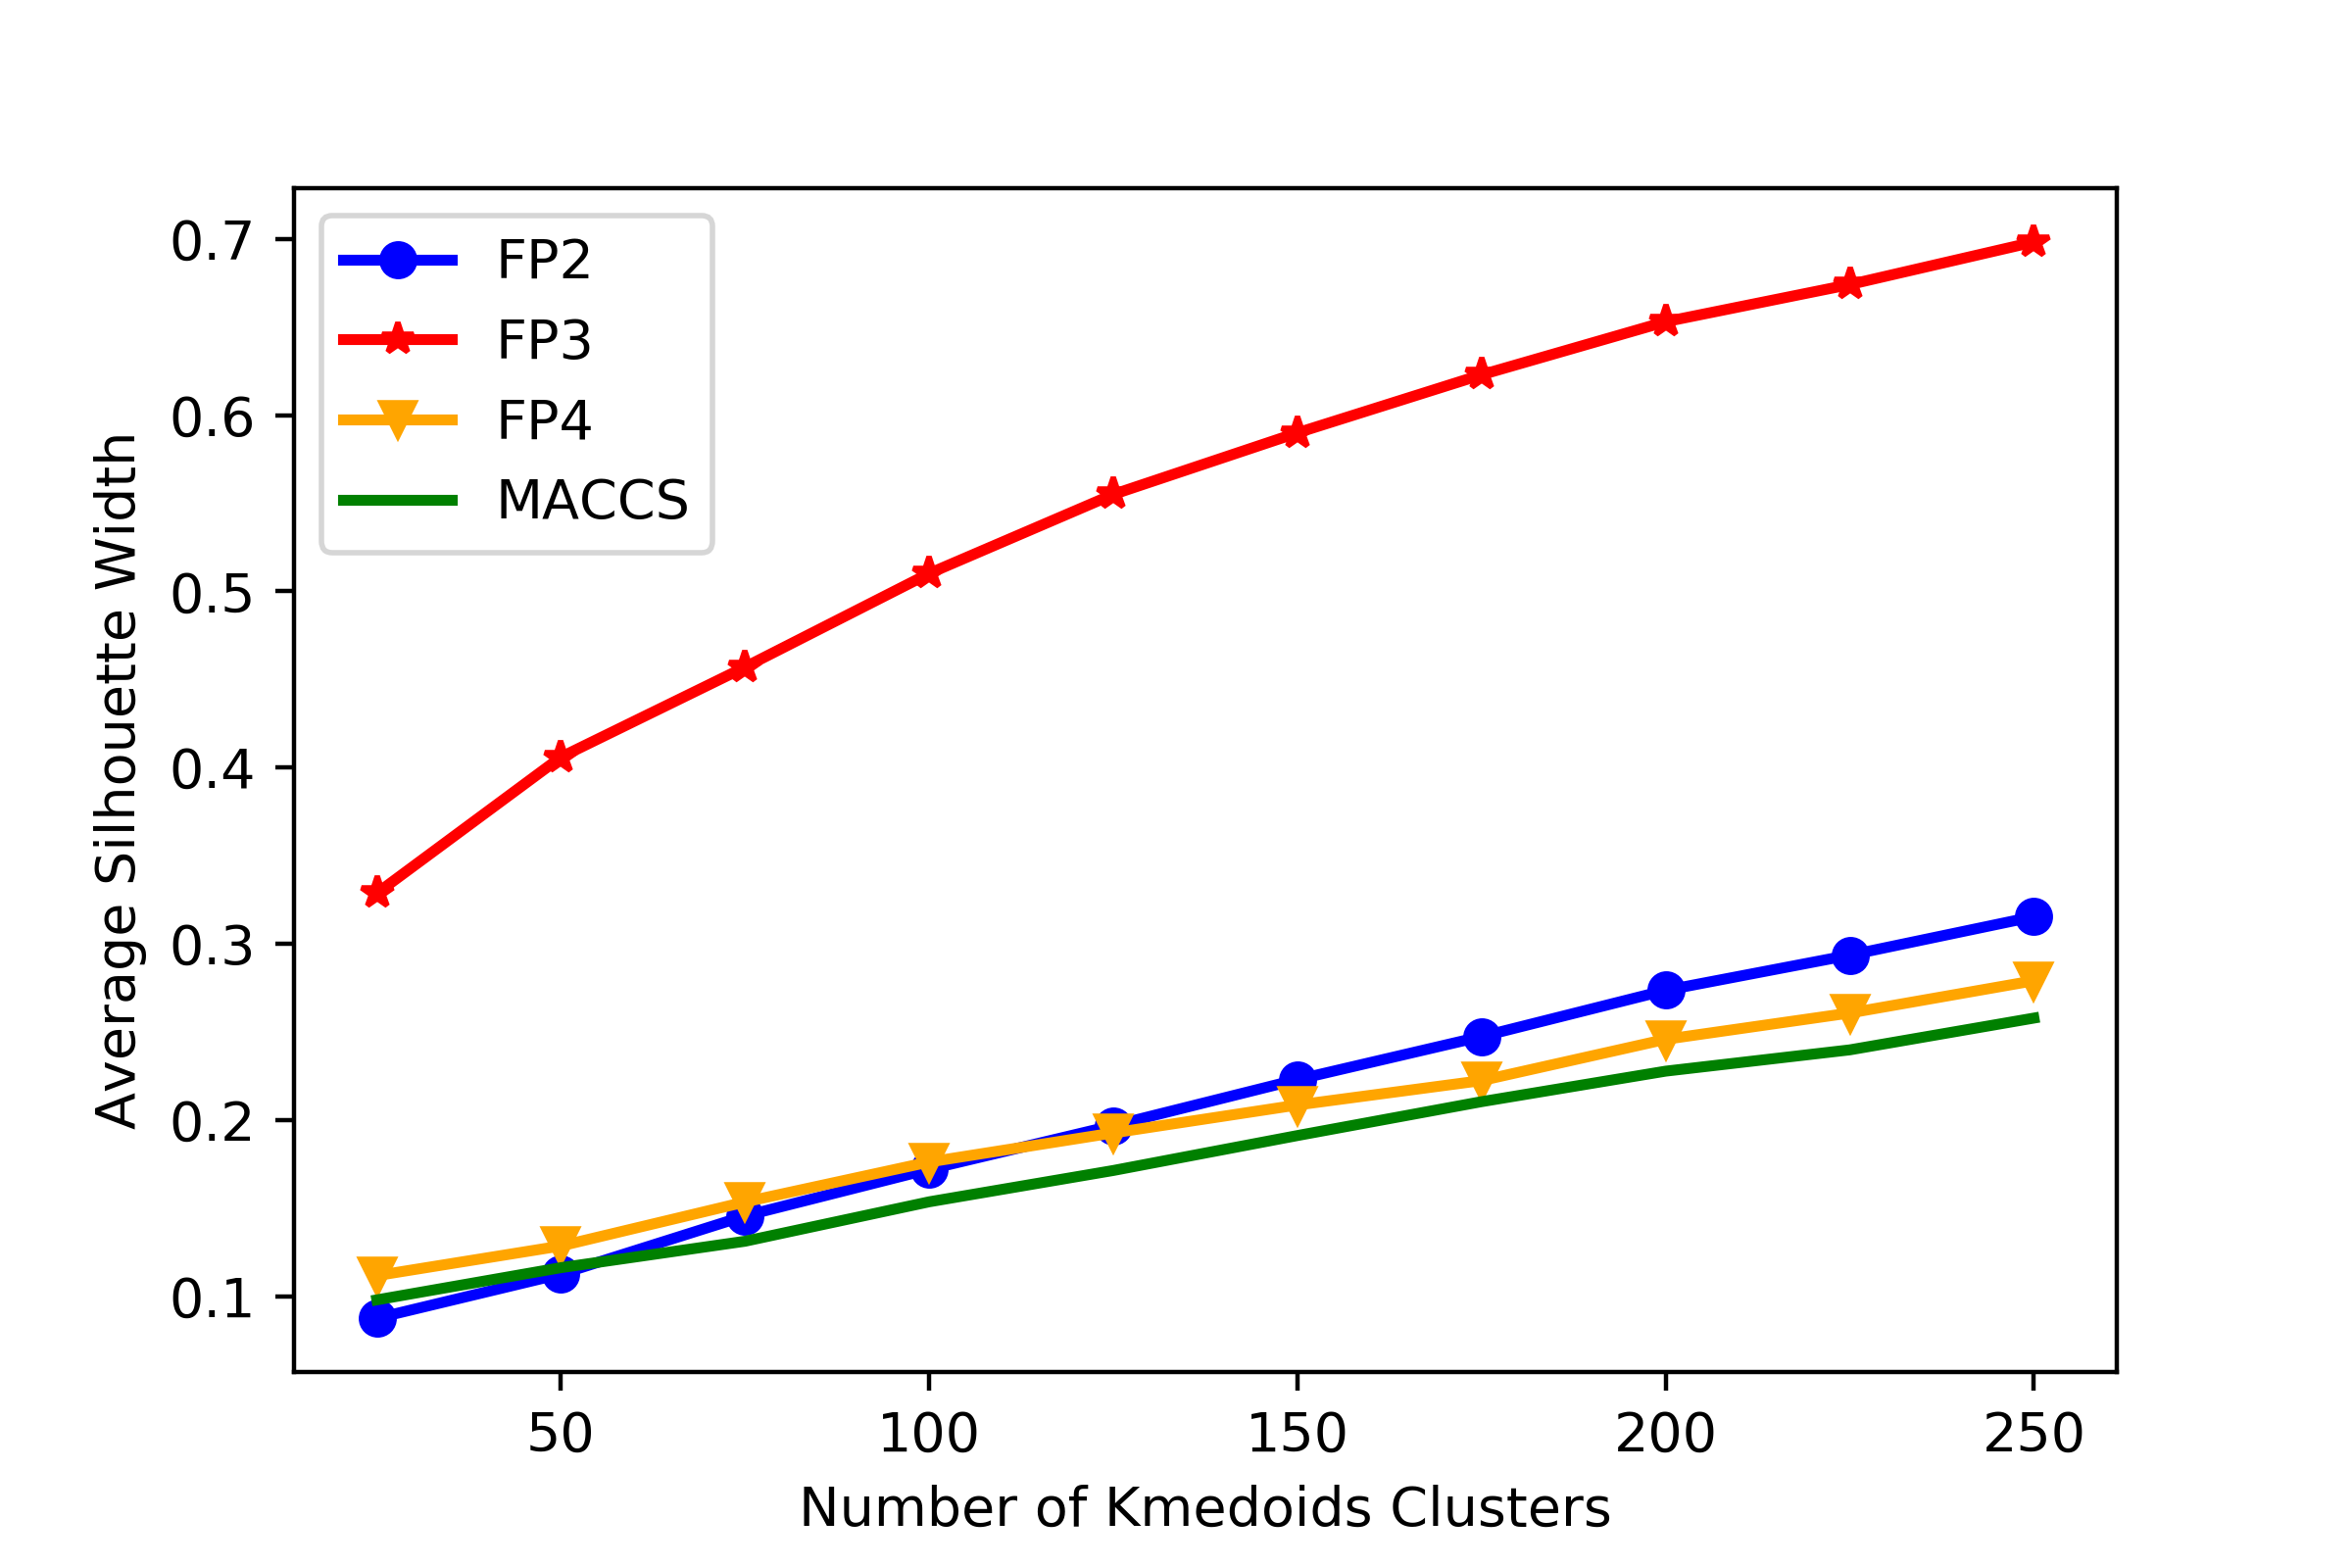
\includegraphics[width=0.85\textwidth]{silwidths_kmed.png}
\caption{Plot of average silhouette width per kmedoids clustering for 4 fingerprint methods. Plot generated using the Python library Matplotlib \cite{matplotlib}.}
\label{silwidths}
\end{figure}

Silhouette plots were generated to determine the best choice of number of clusters. As per \textbf{Figure \ref{silwidths}}, the best fingerprint method to separate the drugs into clusters seems to be FP3 (red, starred curve). The high number of clusters needed to get a good silhouette score, indicates that there are many small clusters of drugs rather than larger clusters of drugs. Furthermore, the FP2, MACCS, and FP4 fingerprints are more likely to distribute molecules evenly in space when compared to the FP3 fingerprint. These results make sense considering how the fingerprints are generated: FP2 analyses all molecule fragments of linear chains of up to 7 atoms, FP3 has 55 SMARTS queries, FP4 has the most SMARTS queries ($\sim$300), and MACCS has 166 SMARTS queries. Ironically, FP3 is the worst fingerprint method but the best option for clustering, as it is less restrictive compared to the other fingerprint methods. Clustering fingerprint dissimilarity matrices can therefore show where there are flaws in a fingerprint method, or (alternatively) they can be used to separate molecule groups based on prioritised SMARTS queries (presence or absence of functional groups/patterns in the molecular structure). It is interesting that MACCS has the smallest slope (green, flat curve) in \textbf{Figure \ref{silwidths}} - making it the best fingerprint for this dataset - especially given that FP4 has roughly twice as many SMARTS queries. 

\begin{table}[H]
\centering
\begin{tabular}{cllll}
\toprule
\textbf{Cut Size} & \textbf{Linkage1} & \textbf{Linkage2} & \textbf{Crand} & \textbf{VI} \\
\midrule
50                & ward.D            & complete          & 0.493          & 1.381       \\
100               & ward.D            & complete          & 0.607          & 1.135       \\
150               & ward.D            & complete          & 0.700          & 0.894       \\
\midrule
50                & ward.D            & average           & 0.349          & 1.568       \\
100               & ward.D            & average           & 0.465          & 1.319       \\
150               & ward.D            & average           & 0.608          & 1.066       \\
\midrule
50                & complete          & average           & 0.526          & 1.313       \\
100               & complete          & average           & 0.612          & 1.021       \\
150               & complete          & average           & 0.672          & 0.802      \\
\bottomrule
\end{tabular}
\caption{Results of comparing linkages for the FP3 fingerprint dataset using hierarchical clustering.}
\label{table-hclust-comp}
\end{table}

Another analysis was done on the FP3 fingerprint dissimilarity matrix using the hclust function in R. 3 sets of linkages: ward.D, complete, and average, were used on 3 cluster sizes (number of cuts to make in the tree) - 50, 100, and 150. The corrected rand (crand, also called adjusted rand index or ARI) and the variation of information (VI) indices were calculated for each pair of results using the cluster.stats function from the fpc R-package \cite{r-fpc}. These results are shown in \textbf{Table \ref{table-hclust-comp}}. Increasing the number of clusters increases the Crand value for each pair of linkages, indicating that they are converging on the same clusters. The two most closely related linkages are ward.D and complete, whereas the two most dissimilar linkages are ward.D and average.

\section{Association Rules Analysis}

Association rules were mined from the dataset. An association rule is a statement $A \implies B$, where $A$ is called the antecedent and $B$ is called the consequent. $A \text{, } B \subset I$, where I is a non-empty set, $A\ne \emptyset \text{, } B\neq \emptyset \text{ and } A\cap B=\emptyset$. To judge the association rules, here are some useful functions: 

\begin{enumerate}
    \item \textbf{support} $s(A\implies B) = P(A,B)$, or the probability of A and B occurring
    \item \textbf{confidence} $c(A\implies B) = P(B|A)$, or the probability of B given that A has occurred
    \item \textbf{lift} $L(A\implies B) = \frac{c(A\implies B)}{P(B)}$, \textbf{standardized lift (``slift")} $\ell (A\implies B) = \frac{L(A\implies B)-\lambda}{\nu - \lambda}$
    ,where\\ \textbf{$\lambda$} = max$(\frac{P(A)+P(B)-1}{P(A)P(B)}, \frac{4s}{(1+s)^2}, \frac{s}{P(A)P(B)},\frac{c}{P(B)})$ and  \textbf{$\nu$} = $\frac{1}{max(P(A),P(B))}$
\end{enumerate}

\subsection{Association Rules Preparation}

First, reviews from Pubchem drugs were extracted into a separate file. Then, the length of the review (in terms of letters) was calculated and given a description (v.short, short, medium, long, and v.long - see \textbf{Table \ref{table-revs}} for length ranges and see \textbf{Figure \ref{revlen-boxplot}} for the distribution). The other columns considered were drugName, condition, and rating, the latter of which was categorised into two groups: 1 for ratings $\geq 7$ and 0 for ratings $< 7$. It should be noted that 870 of the reviews were contaminated by poor html scraping in the conditions column (contained $</span>$ tag). The distribution of drugs and conditions in the Pubchem subset can be found in \textbf{Table \ref{table-drugs-conditions}}. Now, with context of the distribution of the data, the association rules are considered.

\begin{table}[H]
\begin{tabular}{ccccc}
\toprule
\textbf{\begin{tabular}[c]{@{}c@{}}(mean, median)\\ review length\end{tabular}} & \textbf{\begin{tabular}[c]{@{}c@{}}(min, max)\\ review length\end{tabular}} & \textbf{\# rev \textgreater{}= 7} & \textbf{\# rev \textless 7}   & \textbf{\# (drugs, conditions)} \\
\midrule
& & & & \vspace{0.1cm} \\
(345.92, 343)                                                                   & (0, 8262)                                                                   & 118915 (67\%)                     & 57589 (33\%)                  & (2500, 855)                     \\
%\midrule
 & & & & \vspace{0.1cm} \\
\midrule
\textbf{\# v.short {[}0,166)}                                                   & \textbf{\# short {[}166, 282)}                                              & \textbf{\# medium {[}282, 410)}   & \textbf{\# long {[}410, 548)} & \textbf{\# v.long {[}548, inf)} \\
\midrule
35261                                                                           & 35209                                                                       & 35428                             & 35006                         & 35600\\
\bottomrule
\end{tabular}
\caption{From the Pubchem subset of drugs, some summary statistics of the reviews, where review length is given by number of letters, and the number of reviews per description is given.}
\label{table-revs}
\end{table}



\begin{table}[H]
\centering
\begin{tabular}{lrrlrr}
\toprule
\textbf{drugName} & \multicolumn{1}{l}{\textbf{Count}} & \multicolumn{1}{l}{\textbf{(\%)}} & \textbf{condition} & \multicolumn{1}{l}{\textbf{Count}} & \multicolumn{1}{l}{\textbf{(\%)}} \\
\midrule
Levonorgestrel    & 4930                               & 2.8                               & Birth Control      & 23579                              & 13.4                              \\
Etonogestrel      & 4421                               & 2.5                               & Depression         & 11518                              & 6.5                               \\
Nexplanon         & 2892                               & 1.6                               & Anxiety            & 7703                               & 4.4                               \\
Phentermine       & 2085                               & 1.2                               & Pain               & 6446                               & 3.7                               \\
Sertraline        & 1868                               & 1.1                               & Acne               & 5694                               & 3.2                               \\
Escitalopram      & 1747                               & 1.0                               & Bipolar Disorder   & 5531                               & 3.1                               \\
\textit{Other}    & \textit{158561}                    & \textit{89.8}                     & \textit{Other}     & \textit{116033}                    &  \textit{65.7} \\
\bottomrule
\end{tabular}
\caption{Summary of drug names and conditions in the Pubchem dataset.}
\label{table-drugs-conditions}
\end{table}

\subsection{Association Rules Results}

By using the apriori algorithm \cite{apriori-paper}, as implemented using the apriori function from the arules R-package \cite{r-arules}, association rules were generated for the dataset. The std\_lift.R file was used from the class to calculated standardised lift \cite{class-notes-arules}. Without access to medical databases, this type of analysis could be used to determine the drugs for which conditions are prescribed. However, it is more interesting to consider the rules where the drug is given a positive or negative review. It is also important to see if the review length has any association rules. Therefore, the right-hand side (rhs) was set to rating and revLenDesc (Desc for short), as in \textbf{Table \ref{table-arules-params}}.

\begin{table}[H]
\centering
\begin{tabular}{lllll}
\toprule
\textbf{analysis} & \textbf{support} & \textbf{confidence} & \textbf{rhs}   & \textbf{\# rules generated} \\
\midrule
(a)               & 0.01             & 0.8                 & any rating     & 3                           \\
(b)               & 0.005            & 0.6                 & rating=0       & 4                           \\
(c)               & 0.0001           & 0.7                 & any revLenDesc & 10                          \\
(d)               & 0.01             & 0.7                 & None           & 15                          \\
(e)               & 0.0075           & 0.75                & None           & 23      \\
\bottomrule
\end{tabular}
\caption{Parameters and appearances for the apriori function with respect to number of generated rules. The max/min length parameters were set to 2--4 and the default$=$lhs for each case.}
\label{table-arules-params}
\end{table}

\newpage

\begin{wrapfigure}{r}{4.5cm}
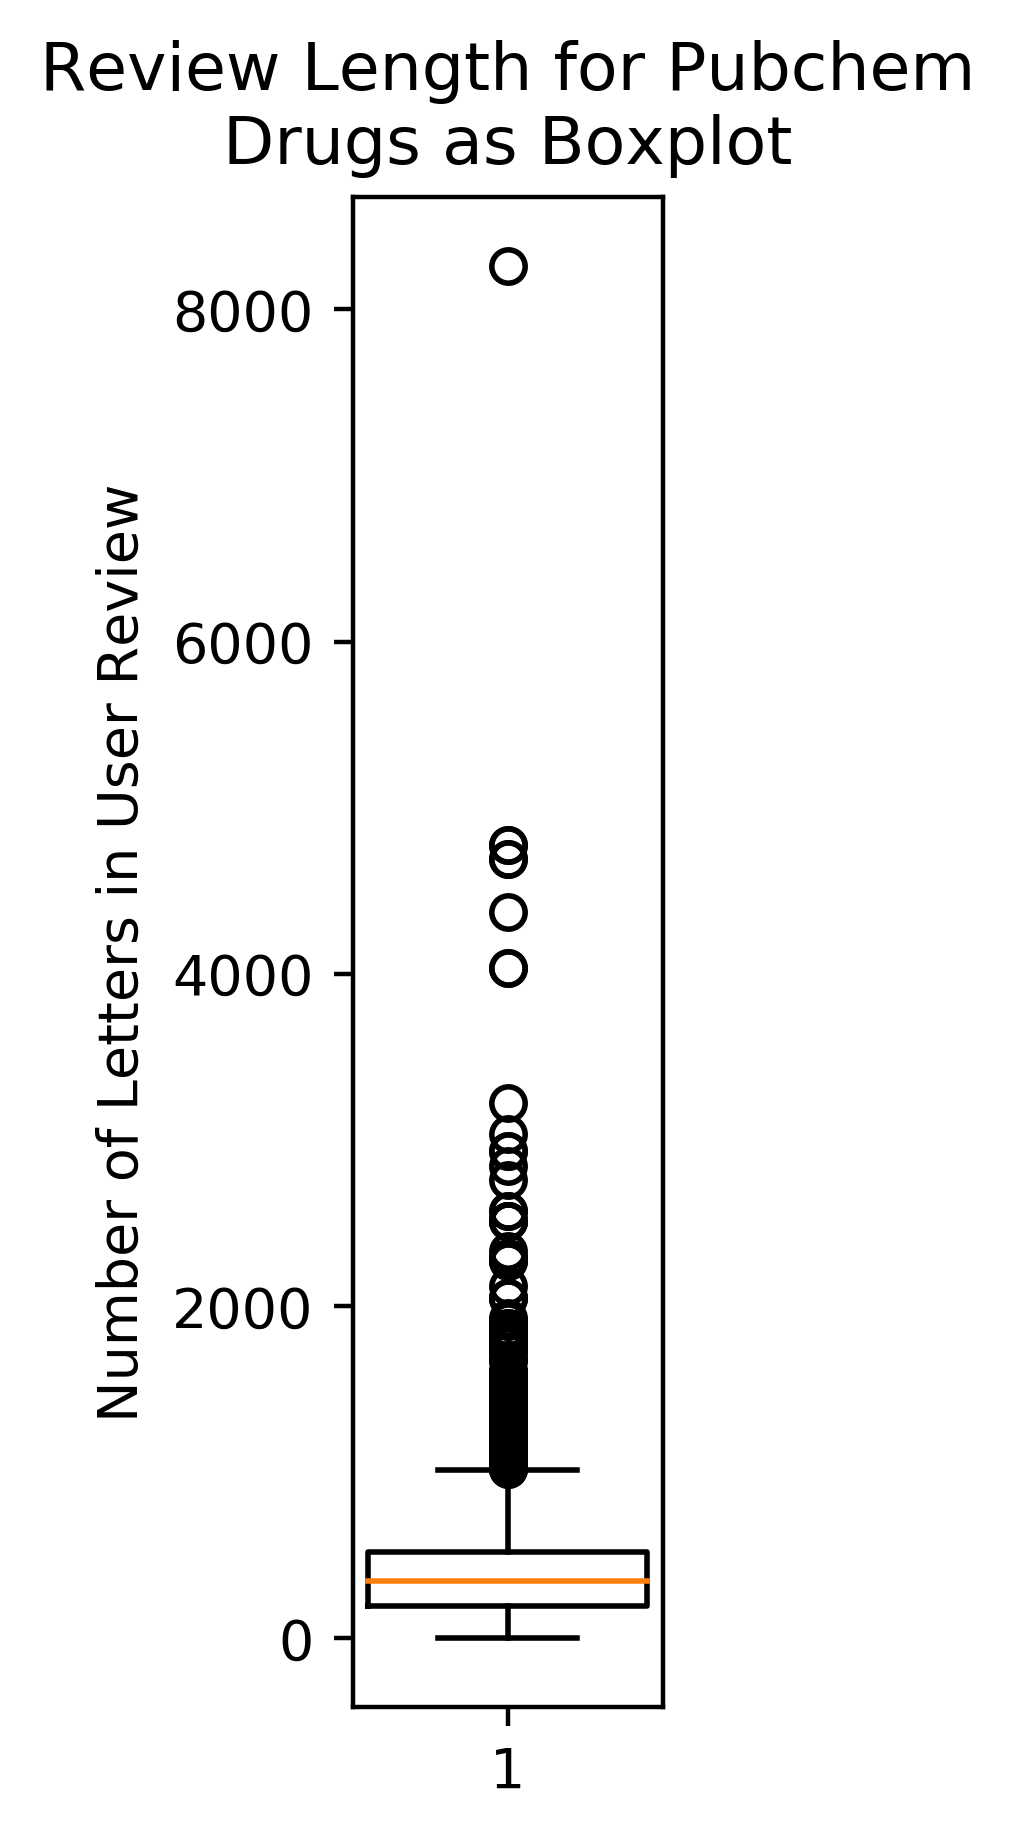
\includegraphics[width=5.2cm]{boxplot_revlen.png}
\caption{Boxplot to show the distribution of review length (in letters) for the Pubchem drugs. Figure generated with Matplotlib \cite{matplotlib}.}
\label{revlen-boxplot}
\end{wrapfigure}

From the results in \textbf{Table \ref{table-arules-results}} for (a), the drugs for smoking cessation and emergency contraception have high confidence, so if a good rating is given it is probable that the drug is for these conditions. The support values for these rules are low, since there are many different drugs and conditions. For the negative ratings in (b), the drug Miconazole and drugs treating Abnormal Uterine Bleeding both get a high count of poor reviews. It makes sense that the number of rules with a rhs of rating=1 is greater than rating=0, since the number of positive reviews in the dataset is about twice the number of negative reviews.

When placing rating descriptions on the rhs in (c), the only description in the top rules was v.short ($<166$ letters). The types of drugs appearing here include pain relievers, acetaminophen, indocin, and naproxen. Notice that there are three rules here where the rating=0, which could mean that users are more likely to leave quick responses for drugs that do not work. The short reviews tied to highly-rated pink eye drugs (first (c) rule - bacterial conjunctivitis) could indicate that the drug is effective and that people don't feel the need to elaborate (perhaps embarrassed). The (d) and (e) columns are mainly to show the types of conditions that often lead to positive reviews; also, there are a couple of times where the description length appears. Instead of v.short category, there are v.long descriptors appearing in the lhs alongside depression, anxiety, and acne. Looking specifically at the types of reviews in the dataset, there are multiple cases where the user will write their life story surrounding their condition (including other drugs they have tried). People who use online media as a way to help with mental health is therefore visible here.

\begin{table}[H]
\centering\small
\begin{adjustwidth}{-50pt}{0pt}
\begin{tabular}{lllllllll}
\toprule
 & \textbf{Rule \#} & \textbf{lhs    =\textgreater{}}                                                                        & \textbf{rhs}           & \textbf{support} & \textbf{confidence} & \textbf{lift} & \textbf{slift} & \textbf{count} \\
 \midrule
\multirow{3}{*}{(a)}                                                   & {[}1{]}                                                             & \{condition= Smoking Cessation\}                                                                       & \{rating=1\}           & 0.01214          & 0.880               & 1.306         & 0.398          & 2142           \\
                                                                       & {[}2{]}                                                             & \{drugName= Phentermine\}                                                                              & \{rating=1\}           & 0.01059          & 0.897               & 1.331         & 0.328          & 1870           \\
                                                                       & {[}3{]}                                                             & \{condition= Emergency Contraception\}                                                                 & \{rating=1\}           & 0.01523          & 0.845               & 1.254         & 0.224          & 2688           \\
\midrule
\multirow{2}{*}{(b)}                                                   & {[}1{]}                                                             & \begin{tabular}[c]{@{}l@{}}\{drugName=Miconazole, \\ Condition= Vaginal Yeast Infection\}\end{tabular} & \{rating=0\}           & 0.00632          & 0.834               & 2.556         & 0.513          & 1116           \\
                                                                       & {[}4{]}                                                             & \{condition= Abnormal Uterine Bleeding\}                                                               & \{rating=0\}           & 0.00776          & 0.694               & 2.128         & 0.236          & 1369           \\
\midrule
\multirow{7}{*}{(c)}                                                   & {[}1{]}                                                             & \begin{tabular}[c]{@{}l@{}}\{condition=Conjunctivitis, Bacterial,\\ Rating=1\}\end{tabular}            & \{Desc=v.short\} & 0.000164         & 0.829               & 4.148         & 0.429          & 29             \\
                                                                       & {[}2{]}                                                             & \{drugName=Acetaminophen\}                                                                             & \{Desc=v.short\} & 0.000176         & 0.795               & 3.979         & 0.316          & 31             \\
                                                                       & {[}6{]}                                                             & \{drugName=Indocin\}                                                                                   & \{Desc=v.short\} & 0.000102         & 0.750               & 3.754         & 0.0551         & 18             \\
                                                                       & {[}7{]}                                                             & \begin{tabular}[c]{@{}l@{}}\{drugName=Naproxen,\\ Condition=Pain,\\ rating=0\}\end{tabular}            & \{Desc=v.short\} & 0.000102         & 0.750               & 3.754         & 0.0551         & 18             \\
                                                                       & {[}8{]}                                                             & \{condition=Extrapyramidal Reaction\}                                                                  & \{Desc=v.short\} & 0.000142         & 0.714               & 3.575         & 0.0476         & 25             \\
                                                                       & {[}9{]}                                                             & \begin{tabular}[c]{@{}l@{}}\{drugName=Aleve,\\ Rating=0\}\end{tabular}                                 & \{Desc=v.short\} & 0.000125         & 0.710               & 3.552         & 0.0323         & 22             \\
                                                                       & {[}10{]}                                                            & \begin{tabular}[c]{@{}l@{}}\{condition=Sciatica,\\ Rating=0\}\end{tabular}                             & \{Desc=v.short\} & 0.000198         & 0.700               & 3.504         & 0              & 35             \\
\midrule
\multirow{8}{*}{(d)}                                                   & {[}8{]}                                                             & \{condition=Weight Loss\}                                                                              & \{rating=1\}           & 0.0219           & 0.797               & 1.183         & 0.322          & 3869           \\
                                                                       & {[}9{]}                                                             & \{condition=Anxiety\}                                                                                  & \{rating=1\}           & 0.0334           & 0.765               & 1.136         & 0.218          & 5895           \\
                                                                       & {[}10{]}                                                            & \{condition=Obesity\}                                                                                  & \{rating=1\}           & 0.0203           & 0.758               & 1.126         & 0.195          & 3575           \\
                                                                       & {[}11{]}                                                            & \{condition=Pain\}                                                                                     & \{rating=1\}           & 0.0276           & 0.756               & 1.123         & 0.188          & 4875           \\
                                                                       & {[}12{]}                                                            & \{condition=Acne\}                                                                                     & \{rating=1\}           & 0.0242           & 0.750               & 1.113         & 0.165          & 4268           \\
                                                                       & {[}13{]}                                                            & \begin{tabular}[c]{@{}l@{}}\{condition=Depression,\\ Desc=v.long\}\end{tabular}                  & \{rating=1\}           & 0.0118           & 0.739               & 1.096         & 0.129          & 2091           \\
                                                                       & {[}14{]}                                                            & \{condition=ADHD\}                                                                                     & \{rating=1\}           & 0.0160           & 0.708               & 1.050704      & 0.0263         & 2828           \\
                                                                       & {[}15{]}                                                            & \begin{tabular}[c]{@{}l@{}}\{condition=Depression,\\ revLenDesc=long\}\end{tabular}                    & \{rating=1\}           & 0.0101           & 0.720               & 1.069072      & 0.0128         & 1774           \\
\midrule
\multirow{5}{*}{(e)}                                                   & {[}12{]}                                                            & \{condition=Panic Disorder\}                                                                           & \{rating=1\}           & 0.00906          & 0.833               & 1.236906      & 0.333          & 1600           \\
                                                                       & {[}13{]}                                                            & \{condition=Migraine\}                                                                                 & \{rating=1\}           & 0.00986          & 0.806               & 1.195676      & 0.222          & 1740           \\
                                                                       & {[}18{]}                                                            & \{drugName=Escitalopram\}                                                                              & \{rating=1\}           & 0.00775          & 0.783               & 1.162281      & 0.104          & 1368           \\
                                                                       & {[}19{]}                                                            & \begin{tabular}[c]{@{}l@{}}\{condition=Anxiety,\\ Desc=v.long\}\end{tabular}                     & \{rating=1\}           & 0.00765          & 0.799               & 1.185673      & 0.0716         & 1350           \\
                                                                       & {[}21{]}                                                            & \begin{tabular}[c]{@{}l@{}}\{condition=Acne,\\ Desc=v.long\}\end{tabular}                        & \{rating=1\}           & 0.00758          & 0.817               & 1.21318       & 0.0454         & 1338          \\
\bottomrule
\end{tabular}
\end{adjustwidth}
\caption{Results for association analysis of drug data for 5 sets of parameters. Rules showing drug-condition relationships or redundant rules have been removed. Results were sorted by slift.}
\label{table-arules-results}
\end{table}


\section{Conclusions}

% Conclusions, in the context of the data and the problem being addressed. [9 marks]

Using the drug dataset, 4 matrices of dissimilarities between drug molecules according to 4 fingerprint measures were generated. The fingerprints were found to be effective in separating the drugs, as a high number of clusters was needed ($>200$) to achieve an average silhouette width of 0.3 as per kmedoids clustering. The worst fingerprint method, and so the best clustering fingerprint, was FP3, which had the fewest SMARTS queries of the methods. With an average silhouette width of $\sim0.7$ and 250 clusters, this would place 1-5 drugs in each cluster for the FP3 fingerprint out of 1370 drugs total. The original drug dataset reported 3654 drugs total, but only 1370 of these drugs had distinct molecular structures, and 1171 of these drugs were not searchable in the Pubchem database.

When comparing ward.D, complete, and average linkages for hierarchical clustering, more cuts led to higher agreement between methods. The best and worst pairs of linkages in terms of agreement were (ward.D, complete) and (ward.D, average) respectively.

When sorting the original dataset, the average text review in the Pubchem subset was found to be $\sim346$ letters, and one person even wrote a short story (8262 letters). Using association rules, short reviews tended to be associated with pain medication and, in some cases, poor reviews of drugs/conditions. Long reviews were tied to mental health issues such as depression. With the highest confidence and support thresholds set, the condition and drug leading to reviews of score 7/10 or higher were smoking cessation and phentermine (weight-loss pill).

















%\footnotesize{\linespread{1}

\printbibliography
%}
\end{document}

% old
\begin{wrapfigure}{r}{5.5cm}
\includegraphics[width=5.5cm]{elbow_labelled.png}
\caption{An elbow plot showing kmeans clustering for up to 200 clusters of FP2 fingerprint data.}
\label{elbowplot}
\end{wrapfigure}

From the elbow plot in \textbf{Figure \ref{elbowplot}}, the optimal number of drug clusters seems to be somewhere between 0 and 50.

A new dataset of drugs was generated using the original data; the new categories are: name, cid, numC, numH, numHetero, molMass, sumFingerprint, drugTarget, drugGroup, medCommentLength, medRating, and sumHelpfulRev.
